\documentclass[conference,compsoc]{IEEEtran}

\usepackage{graphicx}
\usepackage{booktabs}
\usepackage{amsmath}
\usepackage{multirow}
\usepackage{xcolor}
\usepackage{url}
\usepackage{listings}

\lstset{
  basicstyle=\ttfamily\tiny,
  breaklines=true,
  breakatwhitespace=false,
  frame=none,
  columns=fullflexible,
  keepspaces=true,
  xleftmargin=0pt,
  xrightmargin=0pt
}

\begin{document}

\title{Evaluating LLM Reliability for Coding Adversarial Machine Learning Research Papers}

% NO AUTHOR BLOCK - double-blind review

\maketitle

\begin{abstract}
Meta-research on security and machine learning often needs systematic coding of large paper corpora, a task that has stayed manual and slow. Large language models (LLMs) may help automate annotation, but their reliability for coding academic security papers is unknown. We evaluate LLM reliability for coding adversarial ML research by comparing four models (GPT-4o, GPT-5.2, Gemini-3, Claude Sonnet-4.5) to human expert coding on 71 papers and 9 categorical variables. All tested models reach nearly perfect intra-rater consistency (Fleiss' $\kappa = 0.97$--$1.00$), high inter-LLM agreement ($\kappa = 0.79$--$0.85$), and substantial agreement with the human coder ($\kappa = 0.64$--$0.71$). Reliability varies by category: structured variables like domain reach almost perfect agreement ($\kappa = 0.85$), while interpretive ones like attack category are moderate ($\kappa = 0.51$). LLMs are usable as screening tools for structured meta-research in security, though interpretive judgment still benefits from human review.
\end{abstract}

\section{Introduction}

The security and privacy research community increasingly recognizes the need for critical self-reflection on research practices~\cite{metacrisp2026,rossow2012prudent,baset2019analyzing}. From evaluating peer review processes~\cite{soneji2024reflecting} to assessing reproducibility~\cite{olszewski2023reproducibility}, meta-research enables evidence-based improvements to how we conduct, evaluate, and sustain scientific work. Careful meta-analysis still requires someone to code papers: methodology, evaluation practices, artifacts, threat models. That does not scale; manual coding is costly and usually keeps studies to tens of papers.

LLMs have shown decent reliability on text annotation in social science~\cite{gilardi2023chatgpt,tornberg2024chatgpt} and medical reviews~\cite{gartlehner2025ai}, with some agreement levels close to human annotators~\cite{rathje2024gpt}. Nobody has yet tested whether they can reliably code \emph{security} papers, where threat models, evaluation methodology, and jargon are specific. Reliable LLM coding could support large-scale meta-analysis; if not, knowing where they fail clarifies when expert coding is still needed.

Adversarial ML is a good testbed: the field has known evaluation issues~\cite{carlini2017evaluating,athalye2018obfuscated,tramer2020adaptive,arp2022dos} (overstated robustness, weak adaptive evaluation), critiqued in manual work~\cite{carlini2019evaluating} but never in a large systematic coding study. Reliable automated coding would make that kind of meta-analysis feasible.

\textbf{Contribution.} We run the first evaluation of LLM reliability for coding security papers and ask: (1)~How stable is each LLM across repeated codings (intra-rater)? (2)~How well do LLMs match human coders? (3)~Which variables are reliable or brittle under automation?

We use four LLMs (GPT-4o, GPT-5.2, Google Gemini-3, Claude Sonnet-4.5) on 71 adversarial ML papers and 9 categorical variables: research type, domain, venue, artifacts, threat model, and evaluation. Each LLM coded all papers 1--3 times; we compute Fleiss' $\kappa$ for intra-rater and Cohen's $\kappa$ for inter-rater agreement~\cite{krippendorff2004reliability,neuendorf2017content}.

Results are encouraging. All four models achieve nearly perfect self-consistency ($\kappa = 0.97$--$1.00$), high inter-LLM agreement ($\kappa = 0.79$--$0.85$), and substantial agreement with the human coder ($\kappa = 0.64$--$0.71$), in the range often deemed acceptable~\cite{landis1977measurement}. By category, structured variables (e.g., domain $\kappa = 0.85$, threat model $\kappa = 0.75$) reach high agreement, while interpretive ones (e.g., attack category $\kappa = 0.51$) are moderate.

LLMs look useful as \emph{screening} tools for structured variables and could cut human effort on a first pass; they still fall short of expert coding on hard methodological calls. We report reliability numbers and release codebooks, prompts, and scripts for reuse.

\section{Related Work}

\textbf{LLM annotation frameworks.} Recent work demonstrates that LLMs can match or approach human annotator performance on text classification tasks in social science~\cite{gilardi2023chatgpt,tornberg2024chatgpt}, medical systematic reviews~\cite{gartlehner2025ai}, and content moderation~\cite{rathje2024gpt}. Gilardi et al.~\cite{gilardi2023chatgpt} find GPT-3.5 achieves human-level agreement ($\kappa \approx 0.7$) on tweet classification, with GPT-4 outperforming crowd workers. Ziems et al.~\cite{ziems2024can} systematically compare LLMs to human annotators across 27 datasets, finding that LLMs excel on structured tasks but struggle with subjective or culturally-grounded judgments. Our work extends this to \emph{security} papers, where domain-specific jargon, threat models, and evaluation methodology require specialized knowledge.

\textbf{Reliability metrics.} We use Fleiss' $\kappa$ for intra-rater reliability (multi-run models) and Cohen's $\kappa$ for inter-rater reliability, following established content analysis guidelines~\cite{krippendorff2004reliability,neuendorf2017content}. Fleiss' $\kappa$ is only valid for $\geq 3$ raters; we mark single-run models (Sonnet-4.5, Human) as N/A on the diagonal. We report bootstrap 95\% confidence intervals to quantify uncertainty. For threat-model variables (T1/T2), we compute subset $\kappa$ excluding N/A to avoid prevalence inflation, as recommended by Feinstein and Cicchetti~\cite{feinstein1990high}.

\textbf{Security meta-research.} Prior work on adversarial ML evaluation~\cite{carlini2019evaluating,tramer2020adaptive} identifies common pitfalls (weak adaptive attacks, overstated robustness) through manual analysis of select papers. Broader meta-research in security has examined peer review~\cite{soneji2024reflecting}, reproducibility~\cite{olszewski2023reproducibility}, and artifact evaluation~\cite{baset2019analyzing}. These studies typically analyze tens of papers due to manual coding costs. Reliable LLM coding could enable large-scale systematic reviews (hundreds of papers) to quantify trends and identify evaluation gaps across entire subfields.

\subsection{LLM Reliability for Text Annotation}

LLMs have been tested heavily for annotation. Gilardi et al.~\cite{gilardi2023chatgpt} showed ChatGPT beating crowd workers by about 25 points on 6,183 relevance/stance/topic labels. T\"{o}rnberg~\cite{tornberg2024chatgpt} had GPT-4 beat experts and crowd workers on political tweets; Rathje et al.~\cite{rathje2024gpt} got human-like correlations ($r = 0.59$--$0.77$) across 15 datasets and 12 languages ($n = 47{,}925$).

For systematic reviews the picture is mixed. Khraisha et al.~\cite{khraisha2024llm} got adjusted $\kappa = 0.65$ for GPT-4 on screening and extraction, with a tendency to over-exclude. A scoping review of 37 studies~\cite{lieberum2024llm} called LLMs ``not yet ready'' as sole review tools, though about half of studies saw promise for sub-tasks. Gartlehner et al.~\cite{gartlehner2025ai}, on 9,341 extractions from 63 medical studies, found Claude-assisted extraction at 91\% accuracy vs.\ 89\% human-only, with large time savings.

LLM-human agreement depends on the task. In a \emph{Scientific Reports} study~\cite{nature2025comparing}, 8 LLMs and 33 humans did 22,500 annotations: LLMs reached $\alpha \approx 1.00$ on sentiment (above human-human agreement) but both struggled with sarcasm. Ziems et al.~\cite{ziems2024can} reported $\kappa = 0.40$--$0.65$ for 13 LLMs on 25 social-science benchmarks.

Known issues include model drift~\cite{chen2023chatgpt}, prompt sensitivity~\cite{sclar2023quantifying}, and extraction hallucinations. No prior work has evaluated LLM coding of \emph{security} or adversarial ML papers, where technical and methodological nuance differs from general or medical text.

\subsection{Coding Reliability Standards}

Content analysis uses standard agreement metrics. Cohen's $\kappa$~\cite{cohen1960coefficient} handles two raters with chance correction; Fleiss' $\kappa$~\cite{fleiss1971measuring} extends to multiple raters. Krippendorff's $\alpha$~\cite{krippendorff2004reliability} is flexible (any number of coders, levels, missing data); common advice is $\alpha \geq 0.80$ for reliability, with $0.67$--$0.80$ only for tentative use~\cite{hayes2007answering}.

Landis and Koch~\cite{landis1977measurement} label $\kappa = 0.61$--$0.80$ ``substantial'' and $0.81$--$1.0$ ``almost perfect'' (thresholds are conventional). Neuendorf~\cite{neuendorf2017content} suggests $\kappa \geq 0.90$ for broad acceptance and $\geq 0.80$ for published work. Lombard et al.~\cite{lombard2002content} found 31\% of content analyses reported no reliability at all, a gap that shows up often in CS.

LACA~\cite{chew2023llm} outlines a 7-step process for LLM-assisted coding: codebook co-development, face validity, tests that LLM coding is not random, reliability vs.\ humans, phased replacement of manual coding, validation, and reporting. Work on ``scaling hermeneutics''~\cite{epj2025scaling} found that tuning codebooks for LLMs also helped human coders.

\subsection{Meta-Research on Adversarial ML}

Adversarial ML has well-known evaluation problems. Carlini and Wagner~\cite{carlini2017evaluating} showed defensive distillation gave almost no robustness despite 99.5\% claims. Athalye et al.~\cite{athalye2018obfuscated} showed 7 of 9 non-certified ICLR 2018 defenses relied on ``obfuscated gradients''; 6 were later broken. Tram\`{e}r et al.~\cite{tramer2020adaptive} broke 13 more from top venues. Zimmermann et al.~\cite{zimmermann2022increasing} proposed a ``binarization test'' and 11 of 13 defense evaluations failed.

Arp et al.~\cite{arp2022dos} reviewed 30 papers over 10 years and listed 10 pitfalls (data snooping, sampling bias, spurious correlations, lab-only evaluation, etc.). Papernot et al.~\cite{papernot2018sok} described fragmented evaluation language across ML, security, and stats. Grosse et al.~\cite{grosse2023machine} showed academic threat models often mismatch industry needs.

These critiques say \emph{what} is wrong but not \emph{how common} each pattern is. Large-scale coding could answer that, if LLM coding is reliable enough.

\subsection{Reproducibility and Artifacts in Security}

Artifacts and reproducibility are still weak in security. Olszewski et al.~\cite{olszewski2023reproducibility} looked at ~750 ML security papers from top venues (2013--2022) and found no clear gain in artifact availability after artifact-evaluation committees appeared (~2020). In a sample of 171 cybersecurity papers~\cite{dsj2024data}, 89\% had no public code and 58\% no datasets. Venues are tightening rules; USENIX Security 2025 requires artifact submission and can reject for non-compliance~\cite{usenixsec2025artifacts}. Coding when code is released (at vs.\ after publication) helps assess whether such policies work.

\section{Methodology}

We extract 71 adversarial ML papers from top security conferences (IEEE S\&P, CCS, USENIX Security, NDSS), ML venues (ICML, ICLR, NeurIPS), and popular artefacts (CleverHans, RobustBench). The papers are chosen based on their impact and visibility in the adversarial ML literature. An arXiv ID and title identify each paper. We extract full text from each PDF with PyMuPDF. All raters saw the papers in the same order.

Each paper was coded on 9 categorical variables grouped into three themes: research characteristics (G1--G6), threat protection properties specific to attack papers (T1--T2) and practical evaluation (Q1). These coding variables are standard and are commonly seen in the literature in adversarial ML reviews like~\cite{arp2022dos,apruzzese2023real}; our framework was inspired in particular by~\cite{apruzzese2023real}. Table~\ref{tab:codebook} includes the complete variable list and allowed values.

\begin{table*}[t]
\centering
\caption{Coding Schema: 9 Categorical Variables}
\label{tab:codebook}
\small
\begin{tabular}{@{}llp{9cm}@{}}
\toprule
\textbf{Variable} & \textbf{Description} & \textbf{Allowed Values} \\
\midrule
\multicolumn{3}{@{}l}{\textit{Group 1: Research Characteristics}} \\
G1 & Paper type & Attack, Defense, Evaluation, Both, Attack/Defense, Attack/Evaluation, Defense/Evaluation, Attack/Defense/Evaluation \\
G2 & Attack category (if attack) & Evasion, Poisoning, Privacy, Defense, N/A \\
G3 & Application domain & Vision, NLP, LLM, Audio, Malware, Tabular, Cross, Cross-domain \\
G4 & Publication venue category & ML, Security, Journal, arXiv-only \\
G5 & Code currently available & Yes, No \\
G6 & Code release timing & At-pub, Post-pub, Never \\
\midrule
\multicolumn{3}{@{}l}{\textit{Group 2: Threat Model (Attack Papers Only)}} \\
T1 & Adversary model access & White, Black, Gray, White/Black, N/A \\
T2 & Gradient computation required & Yes, No, N/A \\
\midrule
\multicolumn{3}{@{}l}{\textit{Group 3: Practical Evaluation}} \\
Q1 & Evaluation on real-world system & Yes, No, Partial, N/A \\
\bottomrule
\end{tabular}
\end{table*}

We use four LLMs and one human rater (Table~\ref{tab:raters}). Based on their state-of-the-art performance in coding papers, we chose GPT-4o, GPT-5.2, Gemini-3 and Claude Sonnet-4.5 for coding our 71 papers. Each LLM was prompted separately through independent API calls with the same codebook, definition, allowed values, and a 0 temperature for consistency. We made 3 runs for GPT-4o, GPT-5.2 and Gemini-3 each. We performed a single run for Sonnet-4.5 due to the longer length of the prompt associated with the high cost of API calls. A single human rater coded all 71 papers based on the same codebook.

\begin{table}[h]
\centering
\caption{Raters and Run Configuration}
\label{tab:raters}
\small
\begin{tabular}{@{}llcc@{}}
\toprule
\textbf{Rater} & \textbf{Model/Source} & \textbf{Runs} & \textbf{Consensus} \\
\midrule
GPT-4o & OpenAI API & 3 & Majority vote \\
GPT-5.2 & OpenAI API & 3 & Majority vote \\
Gemini-3 & Google Gemini 3.0 Pro & 3 & Majority vote \\
Sonnet-4.5 & claude-sonnet-4-5-20250929 & 1 & N/A \\
Human & Domain expert & 1 & N/A \\
\bottomrule
\end{tabular}
\end{table}

Before computing agreement, we normalised all the values by trimming whitespace, hyphens, underscores, and removing \texttt{None}, \texttt{N/A}, \texttt{null}, and empty values, collapsing them to \texttt{n/a} so that formatting noise does not cause disagreement. We use two standard metrics~\cite{krippendorff2004reliability,neuendorf2017content} to compute agreement. For models with 3 runs, we compute Fleiss' $\kappa$~\cite{fleiss1971measuring} over the three runs with items = paper $\times$ variable. This measures the model self-consistency across different runs. For models with only 1 run (Sonnet-4.5, Human), intra-rater reliability cannot be computed and is marked as N/A. For each pair of raters, we compute Cohen's $\kappa$~\cite{cohen1960coefficient} on coding consensus. We concatenate all 9 columns into 639 labels per rater ($71 \times 9$) for a global $5 \times 5$ matrix (diagonal = Fleiss' $\kappa$ for multi-run models, off-diagonal = Cohen's $\kappa$). We also report mean $\kappa$ per variable (G1--G6, T1--T2, Q1) across pairs to see which codes are stable. Interpretation follows the Landis and Koch~\cite{landis1977measurement} scale: $\kappa < 0.21$ (slight), $0.21$--$0.40$ (fair), $0.41$--$0.60$ (moderate), $0.61$--$0.80$ (substantial), $0.81$--$1.00$ (almost perfect).

\section{Results}

Figure~\ref{fig:heatmap} shows the full agreement matrix. Diagonal entries report intra-rater reliability (Fleiss' $\kappa$); off-diagonal entries report inter-rater agreement (Cohen's $\kappa$). Each $\kappa$ is computed over all 639 labels (71 papers $\times$ 9 variables) for the given rater pair.

\begin{figure}[t]
\centering
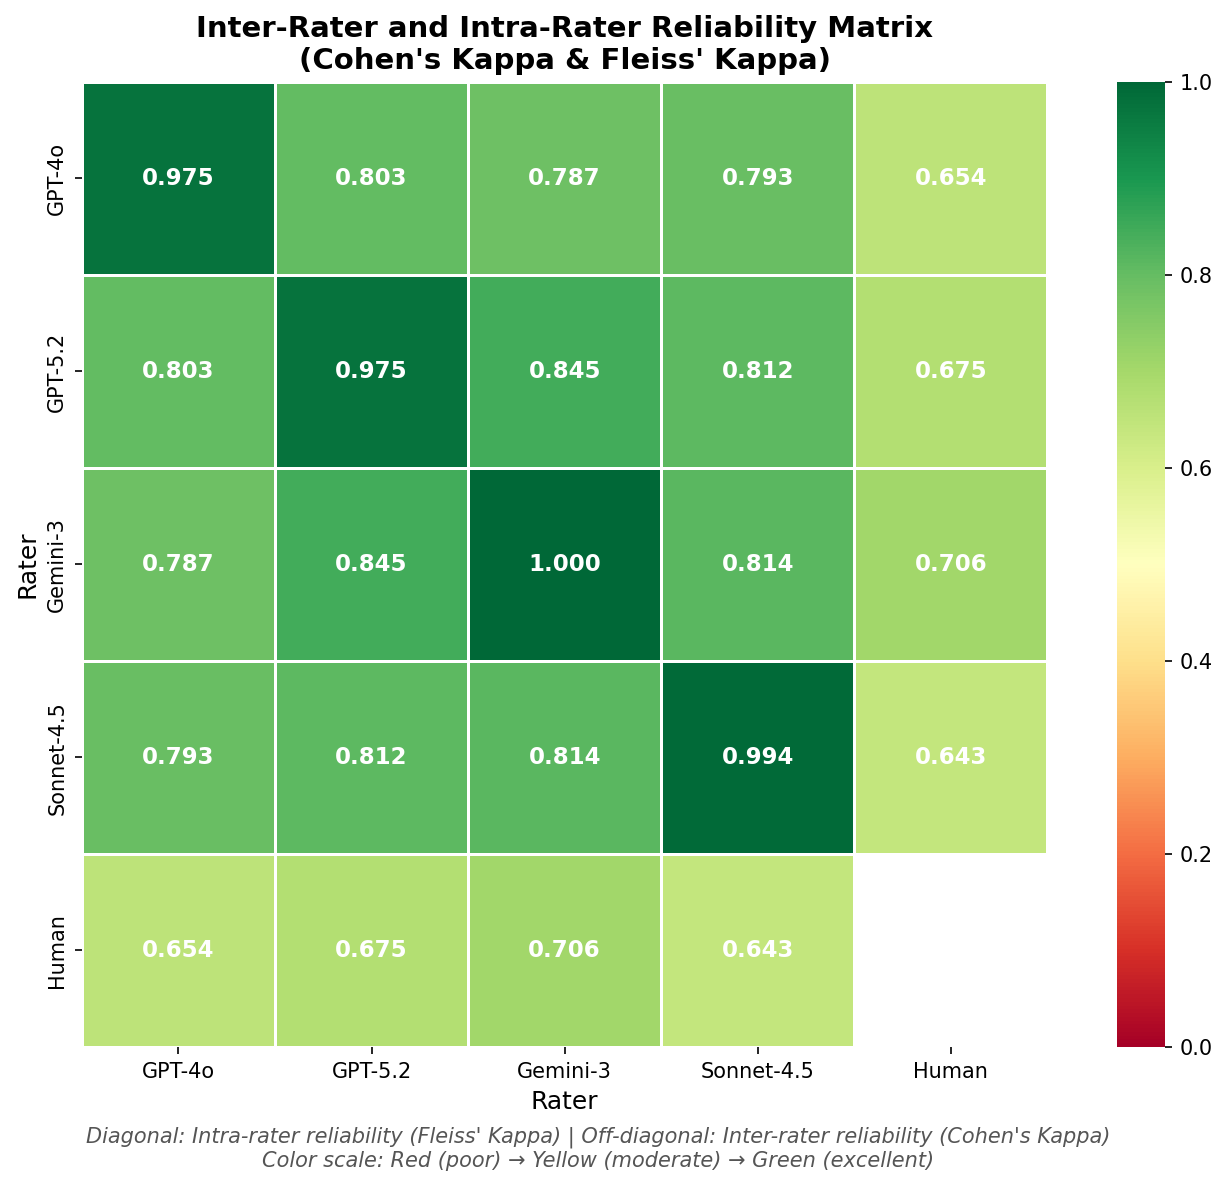
\includegraphics[width=\columnwidth]{reliability_heatmap.png}
\caption{Global agreement matrix. Diagonal (dark green): intra-rater Fleiss' $\kappa$ for models with $\geq$3 runs; N/A for single-run models. Off-diagonal: inter-rater Cohen's $\kappa$. Color scale: red (poor) $\to$ green (excellent).}
\label{fig:heatmap}
\end{figure}

\textbf{Intra-rater reliability.} All multi-run models show nearly perfect self-consistency: Gemini-3 achieves $\kappa = 1.000$ (identical outputs across 3 runs), while GPT-4o and GPT-5.2 both reach $\kappa = 0.975$. Temperature-0 sampling produces highly deterministic behavior.

\textbf{Inter-rater reliability.} All four LLMs show high inter-model agreement ($\kappa = 0.79$--$0.85$), suggesting they converge on similar interpretations. The best LLM pair is GPT-5.2 $\leftrightarrow$ Gemini-3 ($\kappa = 0.846$). Sonnet-4.5 achieves excellent agreement with other LLMs ($\kappa = 0.83$--$0.84$). Critically, all LLMs achieve substantial agreement with the human coder: Gemini-3 ($\kappa = 0.706$), GPT-5.2 ($\kappa = 0.675$), GPT-4o ($\kappa = 0.654$), and Sonnet-4.5 ($\kappa = 0.644$)---all in the ``substantial'' range that Landis and Koch~\cite{landis1977measurement} consider acceptable for published work.

Table~\ref{tab:pervar} shows mean $\kappa$ across all 10 inter-rater pairs, ranked by reliability. Per-variable heatmaps appear in Appendix~\ref{app:heatmaps}.

\begin{table}[h]
\centering
\caption{Per-Variable Agreement (Mean $\kappa$ Across All Pairs with 95\% CI)}
\label{tab:pervar}
\small
\begin{tabular}{@{}llccc@{}}
\toprule
\textbf{Var} & \textbf{Description} & \textbf{Mean $\kappa$} & \textbf{95\% CI} & \textbf{Interpretation} \\
\midrule
G3 & Application domain & .845 & [.796, .887] & Almost perfect \\
G5 & Code available & .776 & [.698, .851] & Substantial \\
T1 & Threat model access & .746 & [.672, .816] & Substantial \\
T2 & Gradient required & .732 & [.643, .816] & Substantial \\
G6 & Code release timing & .732 & [.651, .809] & Substantial \\
\midrule
G4 & Publication venue & .592 & [.463, .717] & Moderate \\
Q1 & Real-world evaluation & .578 & [.476, .676] & Moderate \\
G1 & Paper type & .578 & [.461, .691] & Moderate \\
G2 & Attack category & .514 & [.390, .634] & Moderate \\
\bottomrule
\end{tabular}
\end{table}

\textbf{Structured variables perform best.} Application domain (G3) achieves almost perfect agreement ($\kappa = 0.85$). Threat-model access (T1), gradient requirement (T2), code availability (G5), and release timing (G6) all reach substantial agreement ($\kappa = 0.73$--$0.78$). These have well-defined categories with clear textual signals (e.g., ``white-box,'' ``black-box,'' ``vision,'' ``NLP'').

\textbf{Interpretive variables are harder.} Publication venue (G4), real-world evaluation (Q1), paper type (G1), and attack category (G2) achieve moderate agreement ($\kappa = 0.51$--$0.59$). These require judgment: Is a paper that proposes an attack and then defends against it ``Attack,'' ``Defense,'' or ``Both''? Is a poisoning attack also ``privacy'' if it extracts training data? Disagreements arise from ambiguous boundaries.

The best pairs per variable reach substantial to almost perfect agreement: G3 (domain) achieves $\kappa = 0.87$ (GPT-5.2 $\leftrightarrow$ Sonnet-4.5), T2 (gradient) reaches $\kappa = 0.90$ (GPT-5.2 $\leftrightarrow$ Gemini-3), and G5 (code available) hits $\kappa = 0.89$ (GPT-5.2 $\leftrightarrow$ Gemini-3). Even G2 (attack category) achieves $\kappa = 0.77$ between GPT-5.2 and Sonnet-4.5.

\section{Discussion}

Our results suggest that LLMs are viable for first-pass coding of structured metadata in security meta-research. For variables such as application domain ($\kappa = 0.85$), code availability ($\kappa = 0.78$), and threat model ($\kappa = 0.75$), agreement exceeds inter-human reliability reported in other domains~\cite{ziems2024can}. A practical workflow could employ LLMs to pre-code all papers, with human experts reviewing only disagreements or low-confidence cases.

Notably, all four tested models achieve substantial agreement with the human coder ($\kappa = 0.64$--$0.71$), with no single model dominating across all metrics. Gemini-3 demonstrates a slight advantage, achieving perfect self-consistency ($\kappa = 1.0$), the highest human agreement ($\kappa = 0.706$), and the lowest cost (\$6.66 for 213 codings). The high inter-LLM agreement ($\kappa = 0.79$--$0.85$) suggests that these frontier models converge on similar interpretations of security papers, indicating that the choice of model may matter less than the quality of the codebook and prompt design.

However, interpretive variables remain more challenging. Attack category (G2, $\kappa = 0.51$) and paper type (G1, $\kappa = 0.58$) exhibit lower agreement than structured variables. The codebook permits overlapping labels (e.g., ``Attack/Defense''), and papers frequently span multiple categories. This pattern aligns with findings from social-science annotation~\cite{ziems2024can}, where tasks requiring inference about author intent consistently show lower LLM reliability. For such variables, LLM coding should be treated as a noisy signal that benefits from human adjudication.

These findings carry broader implications for adversarial ML meta-research. Our 71-paper corpus serves as a proof of concept demonstrating that reliable LLM coding could enable systematic studies of evaluation practices, artifact availability, and threat-model reporting across hundreds of papers---the kind of quantitative meta-analysis that manual coding has historically precluded. Researchers could, for instance, track whether artifact-evaluation policies~\cite{usenixsec2025artifacts} correlate with actual code availability over time, or examine whether vulnerabilities such as ``obfuscated gradients''~\cite{athalye2018obfuscated} persist in recent defenses. Our reliability numbers provide the first evidence that such large-scale studies are feasible for structured variables in security research.

\section{Limitations}

\textbf{Statistical methodology.} We report a global $\kappa$ by concatenating all nine variables, which mixes heterogeneous label spaces and prevalences. Per-variable $\kappa$ (Table~\ref{tab:pervar}) provides more granular reliability estimates and should be preferred for interpretation. For T1/T2 (threat model variables), we report subset $\kappa$ excluding N/A to avoid prevalence inflation: LLMs marked 56--68\% of papers as N/A for T1/T2, while the human marked 41--45\%. Critically, T2 (gradient required) shows very low LLM--human agreement ($\kappa = 0.18$--0.33) when N/A is excluded, despite appearing ``substantial'' in the global analysis. This highlights the risk of N/A-driven inflation in threat-model coding.

\textbf{Single human coder.} We use one expert coder due to resource constraints. A single human coder may have bias that could be mitigated by multiple raters with adjudication. Prior work suggests human--human $\kappa$ for similar tasks is 0.6--0.8~\cite{krippendorff2004reliability}; our LLM--human $\kappa = 0.64$--0.71$ is within this range, but validation with multiple humans is needed.

\textbf{Robustness.} High intra-rater $\kappa$ at temperature=0 reflects deterministic sampling, not robustness to prompt variations or context changes. We did not test sensitivity to prompt paraphrasing, few-shot examples, or alternative codebook formulations~\cite{sclar2023quantifying}. Configuration sensitivity (``LLM hacking'') can flip downstream conclusions even with small prompt changes, requiring pre-registration and sensitivity reporting for production meta-research.

\textbf{Codebook ambiguities.} Some categories overlap (e.g., G1 ``Both'' vs ``Attack/Defense''; G2 includes ``Defense'' as an attack category; G3 ``Cross'' vs ``Cross-domain''), contributing to moderate $\kappa$ on interpretive variables. Future work should refine category boundaries and test whether disambiguation improves reliability.

\textbf{Ground-truthing asymmetry.} For G5/G6 (code availability/timing), the human coder may have accessed web resources (GitHub, project pages) while LLMs saw only PDF text (first 15 pages). This information asymmetry may affect LLM--human agreement on these variables and should be controlled in future studies.

\textbf{Generalizability.} We test only a few state-of-the-art models due to API budget constraints. Other models (Opus 4.6, o3 reasoning) may show different results. Model evolution may also change reliability over time~\cite{chen2023chatgpt}. We use a single one-shot prompt without optimization; per-model tuning or few-shot examples could improve reliability. Finally, our adversarial ML corpus may not generalize to other security fields (systems security, cryptography).

\section{Conclusion}

We evaluated LLM reliability for coding adversarial ML papers on 9 categorical variables and found that all models achieve nearly perfect self-consistency ($\kappa = 0.97$--$1.00$) and substantial agreement with a human expert ($\kappa = 0.64$--$0.71$), with reliability varying by variable type: structured codes like domain reach almost perfect agreement ($\kappa = 0.85$), while interpretive codes like attack category are moderate ($\kappa = 0.51$--$0.58$). These results indicate that LLMs are usable as screening tools for structured meta-research in security, though they do not yet replace expert coding for nuanced methodological judgment. All supplementary materials including codebook, prompts, analysis scripts, raw CSV outputs, and per-model coding results are available at: \url{https://github.com/actionproject-madhav/llm-paper-coding-reliability}.

\section{Ethics Considerations}

We evaluate LLM coding of public academic papers. No human subjects; all papers are published and openly or institutionally accessible. No privacy, consent, or harm issues. The goal is to improve how the security community does meta-research.

\section{LLM Usage Considerations}

LLMs were both \emph{evaluated} (as coders) and \emph{used} (literature search, prompts, some analysis). We treat their coding output as data and validate it against human coding. LLMs helped with lit search, LaTeX, and debugging. Some experiment codes are AI-generated with proper human verification.
We release prompts, scripts, and raw outputs for replication.
\bibliographystyle{IEEEtran}
\bibliography{references}

\appendix
\label{app:heatmaps}

\begin{figure*}[t]
\noindent\begin{minipage}[t]{0.48\textwidth}
\textbf{Appendix}

\medskip
Figure~\ref{fig:percolumn} shows Cohen's $\kappa$ for each variable across all rater pairs. Diagonal entries show intra-rater reliability (Fleiss' $\kappa$). Variables G3 (domain), G5 (code available), T1 (threat model), and T2 (gradient) show consistent high agreement across most LLM pairs. Variables G1 (paper type), G2 (attack category), and Q1 (real-world evaluation) show moderate agreement, reflecting their interpretive nature.

\medskip
All LLMs received identical system prompts with temperature set to 0.0 for deterministic outputs. Each paper was provided as extracted PDF text (first 15 pages, max 50,000 characters) with title and arXiv ID.

\medskip
Our corpus comprises 71 adversarial ML papers selected based on adoption in major security artifacts: CleverHans, IBM ART, Foolbox, AutoAttack, RobustBench, TextAttack, HarmBench, PyRIT, and MITRE ATLAS. Papers span 2013--2024 and include foundational attacks (e.g., FGSM, C\&W), robustness benchmarks, certified defenses, and recent LLM jailbreaking work.

\medskip
All supplementary materials are available at our GitHub repository: \url{https://github.com/actionproject-madhav/llm-paper-coding-reliability}, including raw CSV outputs from each model run (3 runs per LLM), human expert codings, the complete paper list with arXiv IDs and PDF links, analysis scripts for computing $\kappa$ statistics, and API interaction code for each model.
\end{minipage}%
\hfill
\begin{minipage}[t]{0.50\textwidth}
\textbf{Coding Prompt}
\begin{lstlisting}
You are coding academic papers for adversarial ML research. For each paper, assign values to exactly 9 variables. Use ONLY the allowed values listed below.

## CODING VARIABLES (STRICT VALUES)

### G1: Paper Type
ALLOWED: "Attack", "Defense", "Evaluation", "Both", "Attack/Defense", "Attack/Evaluation", "Defense/Evaluation", "Attack/Defense/Evaluation"

### G2: Threat Category
ALLOWED: "Evasion", "Poisoning", "Privacy", "Defense", "N/A"

### G3: Domain
ALLOWED: "Vision", "NLP", "LLM", "Audio", "Malware", "Tabular", "Cross", "Cross-domain"

### G4: Publication Venue
ALLOWED: "ML", "Security", "Journal", "arXiv-only"

### G5: Code Available
ALLOWED: "Yes", "No"

### G6: Code Release Timing
ALLOWED: "At-pub", "Post-pub", "Never"

### T1: Model Access Level (attacks only)
ALLOWED: "White", "Black", "Gray", "White/Black", "N/A"

### T2: Gradient Required (attacks only)
ALLOWED: "Yes", "No", "N/A"

### Q1: Real-World Evaluation
ALLOWED: "Yes", "No", "Partial", "N/A"

## OUTPUT FORMAT
Return ONLY valid JSON (no markdown):
{
  "G1": "<value>", "G2": "<value>",
  "G3": "<value>", "G4": "<value>",
  "G5": "<value>", "G6": "<value>",
  "T1": "<value>", "T2": "<value>",
  "Q1": "<value>",
  "reasoning": "Brief explanation"
}

CRITICAL: Use ONLY the allowed values. Do NOT create new values.
\end{lstlisting}
\end{minipage}
\end{figure*}

\begin{figure*}[b]
\centering
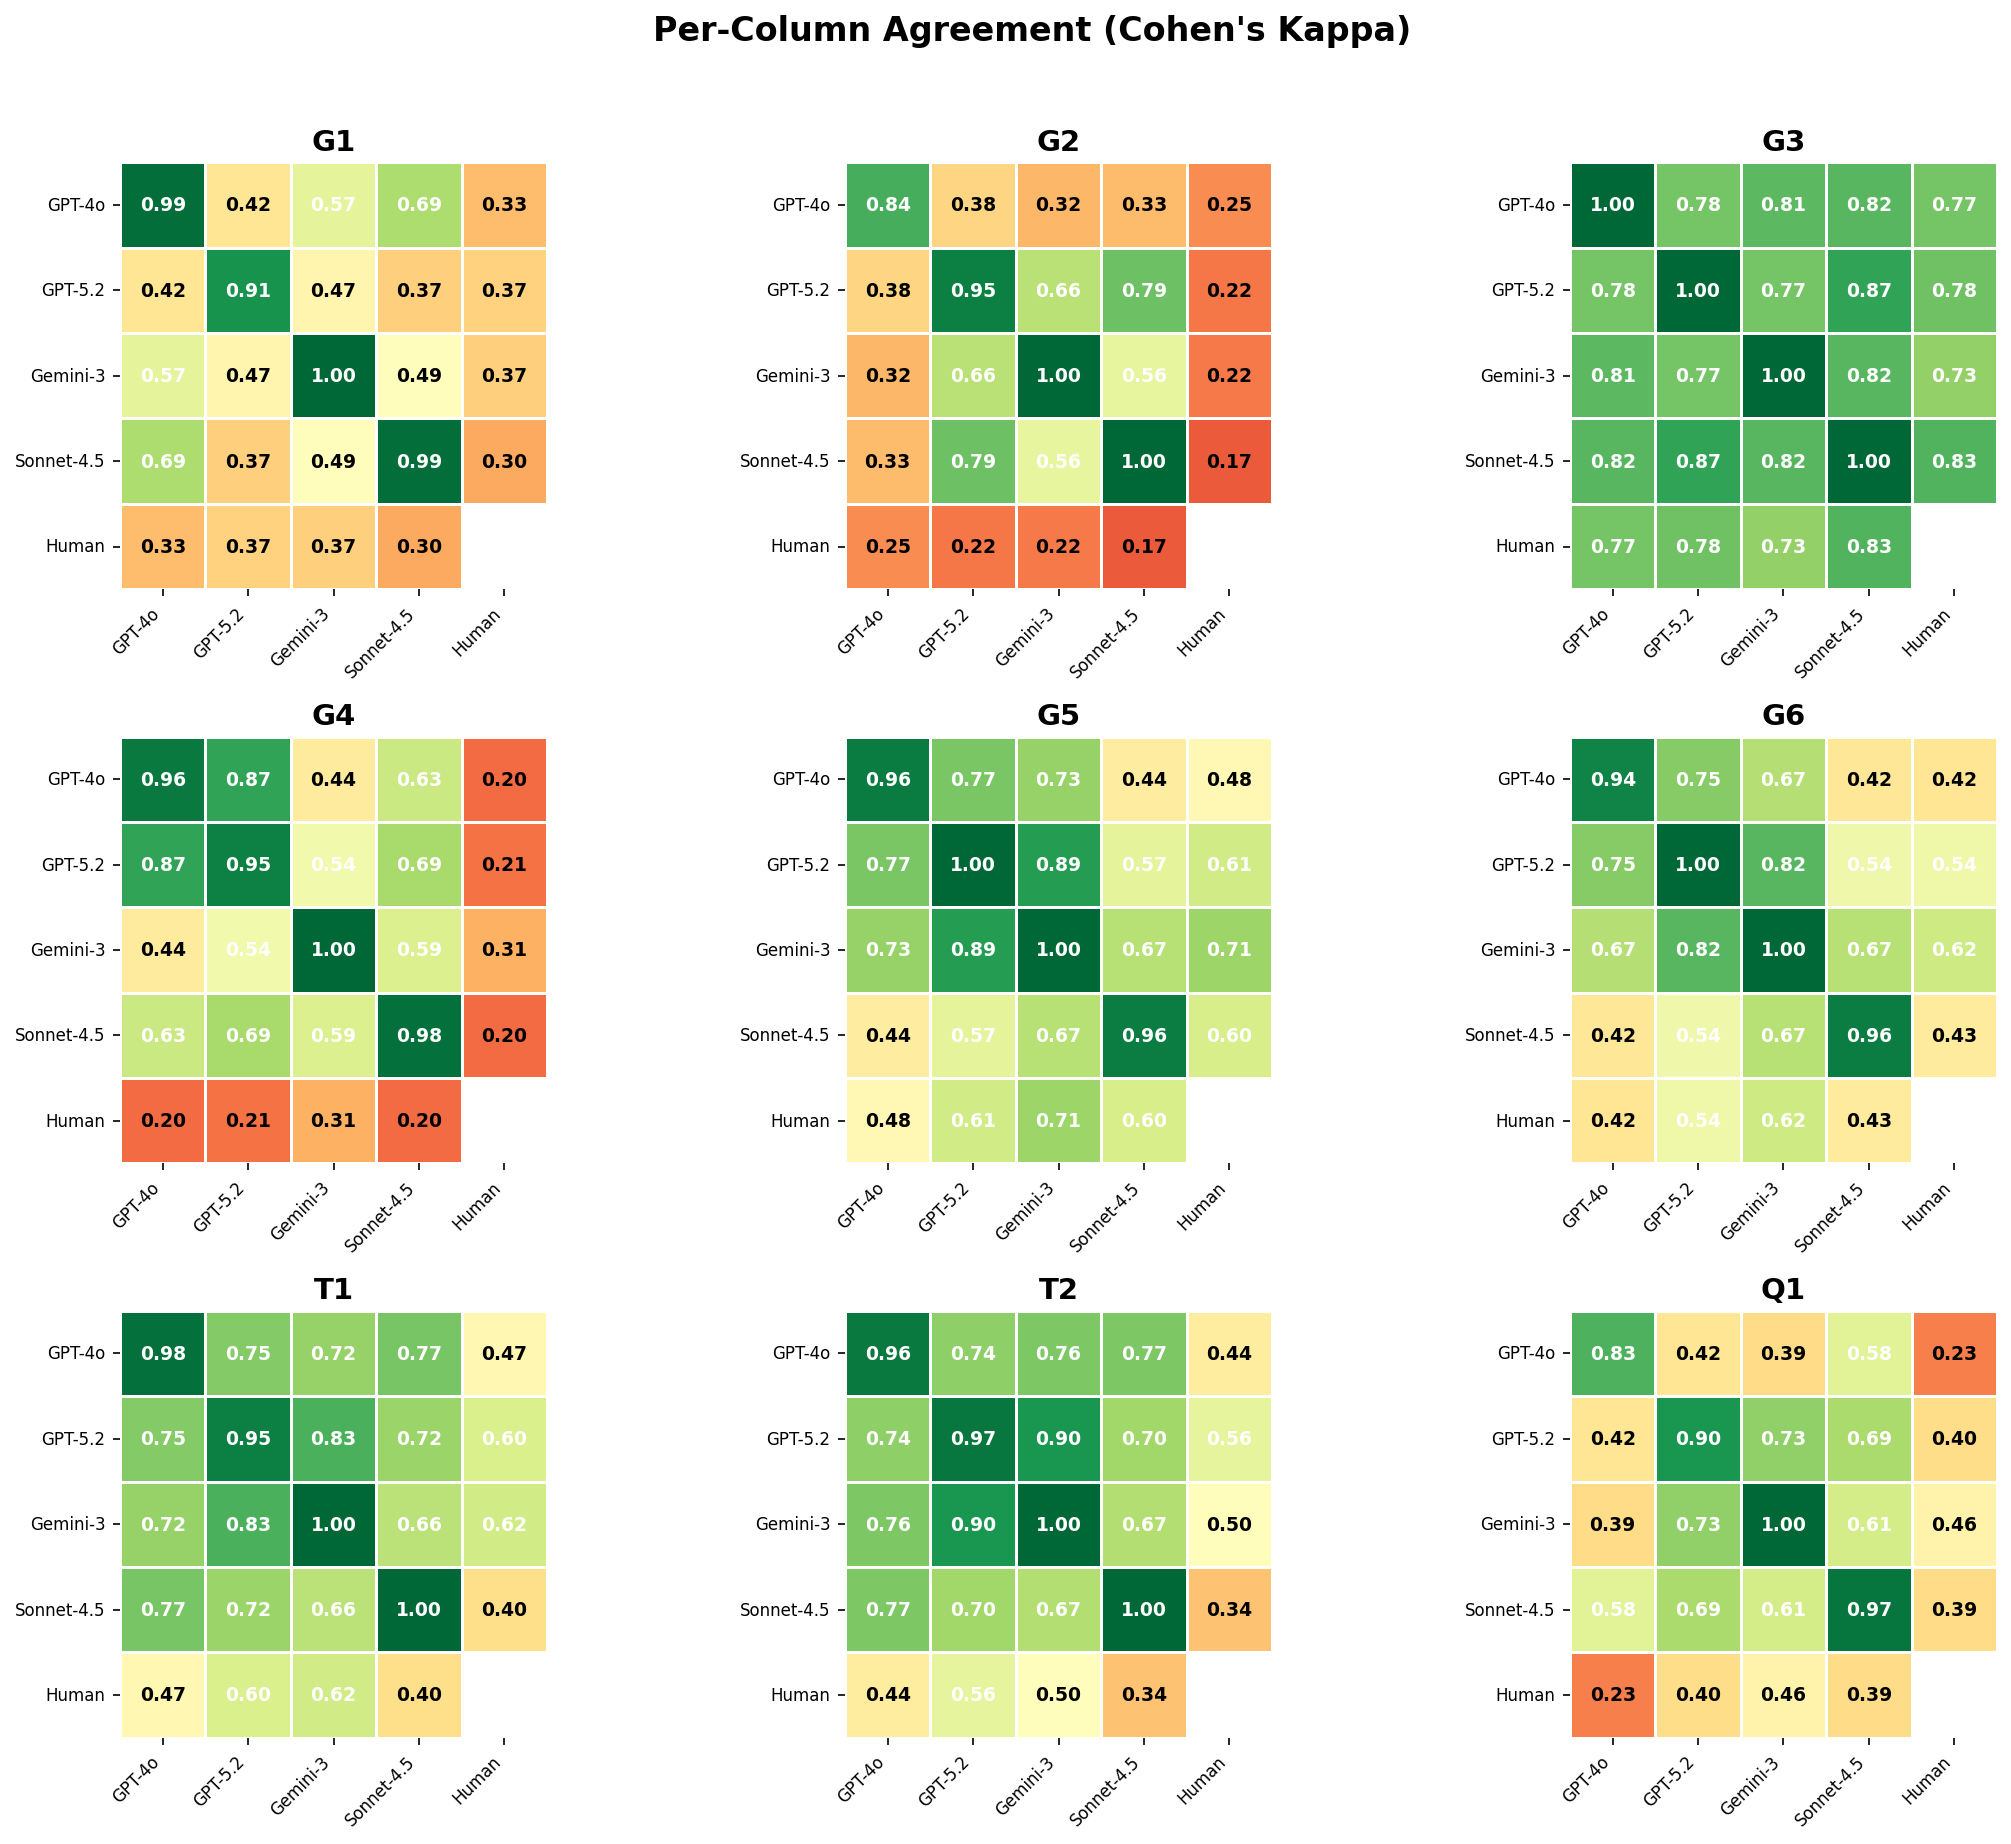
\includegraphics[width=0.82\textwidth]{per_column_heatmaps.png}
\caption{Per-variable agreement heatmaps showing pairwise $\kappa$ for each coding variable (G1--G6: research characteristics; T1--T2: threat model; Q1: evaluation). Diagonal entries show intra-rater Fleiss' $\kappa$. Color scale ranges from red (poor) to green (excellent).}
\label{fig:percolumn}
\end{figure*}

\end{document}
